\documentclass[1p]{elsarticle_modified}
%\bibliographystyle{elsarticle-num}

%\usepackage[colorlinks]{hyperref}
%\usepackage{abbrmath_seonhwa} %\Abb, \Ascr, \Acal ,\Abf, \Afrak
\usepackage{amsfonts}
\usepackage{amssymb}
\usepackage{amsmath}
\usepackage{amsthm}
\usepackage{scalefnt}
\usepackage{amsbsy}
\usepackage{kotex}
\usepackage{caption}
\usepackage{subfig}
\usepackage{color}
\usepackage{graphicx}
\usepackage{xcolor} %% white, black, red, green, blue, cyan, magenta, yellow
\usepackage{float}
\usepackage{setspace}
\usepackage{hyperref}

\usepackage{tikz}
\usetikzlibrary{arrows}

\usepackage{multirow}
\usepackage{array} % fixed length table
\usepackage{hhline}

%%%%%%%%%%%%%%%%%%%%%
\makeatletter
\renewcommand*\env@matrix[1][\arraystretch]{%
	\edef\arraystretch{#1}%
	\hskip -\arraycolsep
	\let\@ifnextchar\new@ifnextchar
	\array{*\c@MaxMatrixCols c}}
\makeatother %https://tex.stackexchange.com/questions/14071/how-can-i-increase-the-line-spacing-in-a-matrix
%%%%%%%%%%%%%%%

\usepackage[normalem]{ulem}

\newcommand{\msout}[1]{\ifmmode\text{\sout{\ensuremath{#1}}}\else\sout{#1}\fi}
%SOURCE: \msout is \stkout macro in https://tex.stackexchange.com/questions/20609/strikeout-in-math-mode

\newcommand{\cancel}[1]{
	\ifmmode
	{\color{red}\msout{#1}}
	\else
	{\color{red}\sout{#1}}
	\fi
}

\newcommand{\add}[1]{
	{\color{blue}\uwave{#1}}
}

\newcommand{\replace}[2]{
	\ifmmode
	{\color{red}\msout{#1}}{\color{blue}\uwave{#2}}
	\else
	{\color{red}\sout{#1}}{\color{blue}\uwave{#2}}
	\fi
}

\newcommand{\Sol}{\mathcal{S}} %segment
\newcommand{\D}{D} %diagram
\newcommand{\A}{\mathcal{A}} %arc


%%%%%%%%%%%%%%%%%%%%%%%%%%%%%5 test

\def\sl{\operatorname{\textup{SL}}(2,\Cbb)}
\def\psl{\operatorname{\textup{PSL}}(2,\Cbb)}
\def\quan{\mkern 1mu \triangleright \mkern 1mu}

\theoremstyle{definition}
\newtheorem{thm}{Theorem}[section]
\newtheorem{prop}[thm]{Proposition}
\newtheorem{lem}[thm]{Lemma}
\newtheorem{ques}[thm]{Question}
\newtheorem{cor}[thm]{Corollary}
\newtheorem{defn}[thm]{Definition}
\newtheorem{exam}[thm]{Example}
\newtheorem{rmk}[thm]{Remark}
\newtheorem{alg}[thm]{Algorithm}

\newcommand{\I}{\sqrt{-1}}
\begin{document}

%\begin{frontmatter}
%
%\title{Boundary parabolic representations of knots up to 8 crossings}
%
%%% Group authors per affiliation:
%\author{Yunhi Cho} 
%\address{Department of Mathematics, University of Seoul, Seoul, Korea}
%\ead{yhcho@uos.ac.kr}
%
%
%\author{Seonhwa Kim} %\fnref{s_kim}}
%\address{Center for Geometry and Physics, Institute for Basic Science, Pohang, 37673, Korea}
%\ead{ryeona17@ibs.re.kr}
%
%\author{Hyuk Kim}
%\address{Department of Mathematical Sciences, Seoul National University, Seoul 08826, Korea}
%\ead{hyukkim@snu.ac.kr}
%
%\author{Seokbeom Yoon}
%\address{Department of Mathematical Sciences, Seoul National University, Seoul, 08826,  Korea}
%\ead{sbyoon15@snu.ac.kr}
%
%\begin{abstract}
%We find all boundary parabolic representation of knots up to 8 crossings.
%
%\end{abstract}
%\begin{keyword}
%    \MSC[2010] 57M25 
%\end{keyword}
%
%\end{frontmatter}

%\linenumbers
%\tableofcontents
%
\newcommand\colored[1]{\textcolor{white}{\rule[-0.35ex]{0.8em}{1.4ex}}\kern-0.8em\color{red} #1}%
%\newcommand\colored[1]{\textcolor{white}{ #1}\kern-2.17ex	\textcolor{white}{ #1}\kern-1.81ex	\textcolor{white}{ #1}\kern-2.15ex\color{red}#1	}

{\Large $\underline{12a_{1285}~(K12a_{1285})}$}

\setlength{\tabcolsep}{10pt}
\renewcommand{\arraystretch}{1.6}
\vspace{1cm}\begin{tabular}{m{100pt}>{\centering\arraybackslash}m{274pt}}
\multirow{5}{120pt}{
	\centering
	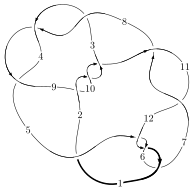
\includegraphics[width=112pt]{../../../GIT/diagram.site/Diagrams/png/2086_12a_1285.png}\\
\ \ \ A knot diagram\footnotemark}&
\allowdisplaybreaks
\textbf{Linearized knot diagam} \\
\cline{2-2}
 &
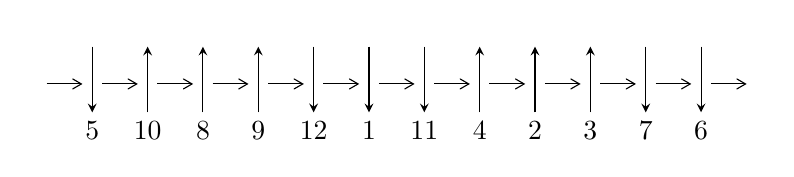
\begin{tikzpicture}[x=20pt, y=17pt]
	% nodes
	\node (C0) at (0, 0) {};
	\node (C1) at (1, 0) {};
	\node (C1U) at (1, +1) {};
	\node (C1D) at (1, -1) {5};

	\node (C2) at (2, 0) {};
	\node (C2U) at (2, +1) {};
	\node (C2D) at (2, -1) {10};

	\node (C3) at (3, 0) {};
	\node (C3U) at (3, +1) {};
	\node (C3D) at (3, -1) {8};

	\node (C4) at (4, 0) {};
	\node (C4U) at (4, +1) {};
	\node (C4D) at (4, -1) {9};

	\node (C5) at (5, 0) {};
	\node (C5U) at (5, +1) {};
	\node (C5D) at (5, -1) {12};

	\node (C6) at (6, 0) {};
	\node (C6U) at (6, +1) {};
	\node (C6D) at (6, -1) {1};

	\node (C7) at (7, 0) {};
	\node (C7U) at (7, +1) {};
	\node (C7D) at (7, -1) {11};

	\node (C8) at (8, 0) {};
	\node (C8U) at (8, +1) {};
	\node (C8D) at (8, -1) {4};

	\node (C9) at (9, 0) {};
	\node (C9U) at (9, +1) {};
	\node (C9D) at (9, -1) {2};

	\node (C10) at (10, 0) {};
	\node (C10U) at (10, +1) {};
	\node (C10D) at (10, -1) {3};

	\node (C11) at (11, 0) {};
	\node (C11U) at (11, +1) {};
	\node (C11D) at (11, -1) {7};

	\node (C12) at (12, 0) {};
	\node (C12U) at (12, +1) {};
	\node (C12D) at (12, -1) {6};
	\node (C13) at (13, 0) {};

	% arrows
	\draw[->,>={angle 60}]
	(C0) edge (C1) (C1) edge (C2) (C2) edge (C3) (C3) edge (C4) (C4) edge (C5) (C5) edge (C6) (C6) edge (C7) (C7) edge (C8) (C8) edge (C9) (C9) edge (C10) (C10) edge (C11) (C11) edge (C12) (C12) edge (C13) ;	\draw[->,>=stealth]
	(C1U) edge (C1D) (C2D) edge (C2U) (C3D) edge (C3U) (C4D) edge (C4U) (C5U) edge (C5D) (C6U) edge (C6D) (C7U) edge (C7D) (C8D) edge (C8U) (C9D) edge (C9U) (C10D) edge (C10U) (C11U) edge (C11D) (C12U) edge (C12D) ;
	\end{tikzpicture} \\
\hhline{~~} \\& 
\textbf{Solving Sequence} \\ \cline{2-2} 
 &
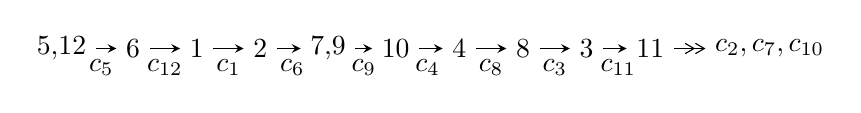
\begin{tikzpicture}[x=23pt, y=7pt]
	% node
	\node (A0) at (-1/8, 0) {5,12};
	\node (A1) at (1, 0) {6};
	\node (A2) at (2, 0) {1};
	\node (A3) at (3, 0) {2};
	\node (A4) at (65/16, 0) {7,9};
	\node (A5) at (41/8, 0) {10};
	\node (A6) at (49/8, 0) {4};
	\node (A7) at (57/8, 0) {8};
	\node (A8) at (65/8, 0) {3};
	\node (A9) at (73/8, 0) {11};
	\node (C1) at (1/2, -1) {$c_{5}$};
	\node (C2) at (3/2, -1) {$c_{12}$};
	\node (C3) at (5/2, -1) {$c_{1}$};
	\node (C4) at (7/2, -1) {$c_{6}$};
	\node (C5) at (37/8, -1) {$c_{9}$};
	\node (C6) at (45/8, -1) {$c_{4}$};
	\node (C7) at (53/8, -1) {$c_{8}$};
	\node (C8) at (61/8, -1) {$c_{3}$};
	\node (C9) at (69/8, -1) {$c_{11}$};
	\node (A10) at (11, 0) {$c_{2},c_{7},c_{10}$};

	% edge
	\draw[->,>=stealth]	
	(A0) edge (A1) (A1) edge (A2) (A2) edge (A3) (A3) edge (A4) (A4) edge (A5) (A5) edge (A6) (A6) edge (A7) (A7) edge (A8) (A8) edge (A9) ;
	\draw[->>,>={angle 60}]	
	(A9) edge (A10);
\end{tikzpicture} \\ 

\end{tabular} \\

\footnotetext{
The image of knot diagram is generated by the software ``\textbf{Draw programme}" developed by Andrew Bartholomew(\url{http://www.layer8.co.uk/maths/draw/index.htm\#Running-draw}), where we modified some parts for our purpose(\url{https://github.com/CATsTAILs/LinksPainter}).
}\phantom \\ \newline 
\centering \textbf{Ideals for irreducible components\footnotemark of $X_{\text{par}}$} 
 
\begin{align*}
I^u_{1}&=\langle 
- u^{23}+2 u^{22}+\cdots+b-1,\;-7 u^{23}+13 u^{22}+\cdots+2 a-12,\;u^{24}-3 u^{23}+\cdots-6 u-2\rangle \\
I^u_{2}&=\langle 
-10 u^{13} a+21 u^{13}+\cdots-17 a+30,\;-2 u^{13} a+2 u^{13}+\cdots-2 a+2,\\
\phantom{I^u_{2}}&\phantom{= \langle  }u^{14}+u^{13}-5 u^{12}-4 u^{11}+10 u^{10}+5 u^9-7 u^8+2 u^7-4 u^6-8 u^5+8 u^4+2 u^3-2 u^2+3 u-1\rangle \\
I^u_{3}&=\langle 
b+1,\;2 u^3-3 u^2+3 a-3 u+3,\;u^4-3 u^2+3\rangle \\
I^u_{4}&=\langle 
b-1,\;- u^2+a+u+1,\;u^4- u^2-1\rangle \\
\\
I^v_{1}&=\langle 
a,\;b+1,\;v+1\rangle \\
\end{align*}
\raggedright * 5 irreducible components of $\dim_{\mathbb{C}}=0$, with total 61 representations.\\
\footnotetext{All coefficients of polynomials are rational numbers. But the coefficients are sometimes approximated in decimal forms when there is not enough margin.}
\newpage
\renewcommand{\arraystretch}{1}
\centering \section*{I. $I^u_{1}= \langle - u^{23}+2 u^{22}+\cdots+b-1,\;-7 u^{23}+13 u^{22}+\cdots+2 a-12,\;u^{24}-3 u^{23}+\cdots-6 u-2 \rangle$}
\flushleft \textbf{(i) Arc colorings}\\
\begin{tabular}{m{7pt} m{180pt} m{7pt} m{180pt} }
\flushright $a_{5}=$&$\begin{pmatrix}1\\0\end{pmatrix}$ \\
\flushright $a_{12}=$&$\begin{pmatrix}0\\u\end{pmatrix}$ \\
\flushright $a_{6}=$&$\begin{pmatrix}1\\u^2\end{pmatrix}$ \\
\flushright $a_{1}=$&$\begin{pmatrix}- u\\- u^3+u\end{pmatrix}$ \\
\flushright $a_{2}=$&$\begin{pmatrix}u^3-2 u\\- u^3+u\end{pmatrix}$ \\
\flushright $a_{7}=$&$\begin{pmatrix}- u^2+1\\- u^4+2 u^2\end{pmatrix}$ \\
\flushright $a_{9}=$&$\begin{pmatrix}\frac{7}{2} u^{23}-\frac{13}{2} u^{22}+\cdots+\frac{37}{2} u+6\\u^{23}-2 u^{22}+\cdots+5 u+1\end{pmatrix}$ \\
\flushright $a_{10}=$&$\begin{pmatrix}\frac{5}{2} u^{23}-\frac{9}{2} u^{22}+\cdots+\frac{25}{2} u+4\\u^{23}-2 u^{22}+\cdots+4 u+1\end{pmatrix}$ \\
\flushright $a_{4}=$&$\begin{pmatrix}-\frac{1}{2} u^{23}+\frac{1}{2} u^{22}+\cdots-\frac{17}{2} u^2-\frac{7}{2} u\\u^{23}- u^{22}+\cdots+4 u+1\end{pmatrix}$ \\
\flushright $a_{8}=$&$\begin{pmatrix}- u^8+3 u^6-3 u^4+1\\- u^{10}+4 u^8-5 u^6+3 u^2\end{pmatrix}$ \\
\flushright $a_{3}=$&$\begin{pmatrix}-\frac{1}{2} u^{23}+\frac{1}{2} u^{22}+\cdots-\frac{13}{2} u-1\\2 u^{23}-3 u^{22}+\cdots+12 u+3\end{pmatrix}$ \\
\flushright $a_{11}=$&$\begin{pmatrix}u^5-2 u^3+u\\u^7-3 u^5+2 u^3+u\end{pmatrix}$\\&\end{tabular}
\flushleft \textbf{(ii) Obstruction class $= -1$}\\~\\
\flushleft \textbf{(iii) Cusp Shapes $= 2 u^{21}-16 u^{19}-6 u^{18}+54 u^{17}+42 u^{16}-82 u^{15}-120 u^{14}+4 u^{13}+148 u^{12}+172 u^{11}+4 u^{10}-204 u^9-204 u^8-20 u^7+146 u^6+168 u^5+66 u^4-40 u^3-76 u^2-56 u-12$}\\~\\
\newpage\renewcommand{\arraystretch}{1}
\flushleft \textbf{(iv) u-Polynomials at the component}\newline \\
\begin{tabular}{m{50pt}|m{274pt}}
Crossings & \hspace{64pt}u-Polynomials at each crossing \\
\hline $$\begin{aligned}c_{1},c_{7},c_{11}\end{aligned}$$&$\begin{aligned}
&u^{24}+9 u^{23}+\cdots-194 u-22
\end{aligned}$\\
\hline $$\begin{aligned}c_{2},c_{3},c_{4}\\c_{8},c_{9},c_{10}\end{aligned}$$&$\begin{aligned}
&u^{24}+u^{23}+\cdots- u+1
\end{aligned}$\\
\hline $$\begin{aligned}c_{5},c_{6},c_{12}\end{aligned}$$&$\begin{aligned}
&u^{24}-3 u^{23}+\cdots-6 u-2
\end{aligned}$\\
\hline
\end{tabular}\\~\\
\newpage\renewcommand{\arraystretch}{1}
\flushleft \textbf{(v) Riley Polynomials at the component}\newline \\
\begin{tabular}{m{50pt}|m{274pt}}
Crossings & \hspace{64pt}Riley Polynomials at each crossing \\
\hline $$\begin{aligned}c_{1},c_{7},c_{11}\end{aligned}$$&$\begin{aligned}
&y^{24}+25 y^{23}+\cdots+1744 y+484
\end{aligned}$\\
\hline $$\begin{aligned}c_{2},c_{3},c_{4}\\c_{8},c_{9},c_{10}\end{aligned}$$&$\begin{aligned}
&y^{24}-33 y^{23}+\cdots-3 y+1
\end{aligned}$\\
\hline $$\begin{aligned}c_{5},c_{6},c_{12}\end{aligned}$$&$\begin{aligned}
&y^{24}-19 y^{23}+\cdots+32 y+4
\end{aligned}$\\
\hline
\end{tabular}\\~\\
\newpage\flushleft \textbf{(vi) Complex Volumes and Cusp Shapes}
$$\begin{array}{c|c|c}  
\text{Solutions to }I^u_{1}& \I (\text{vol} + \sqrt{-1}CS) & \text{Cusp shape}\\
 \hline 
\begin{aligned}
u &= -0.067210 + 0.918173 I \\
a &= \phantom{-}2.61385 - 0.53592 I \\
b &= -1.64955 - 0.33368 I\end{aligned}
 & -18.9666 + 8.2466 I & \phantom{-}9.52974 - 3.63812 I \\ \hline\begin{aligned}
u &= -0.067210 - 0.918173 I \\
a &= \phantom{-}2.61385 + 0.53592 I \\
b &= -1.64955 + 0.33368 I\end{aligned}
 & -18.9666 - 8.2466 I & \phantom{-}9.52974 + 3.63812 I \\ \hline\begin{aligned}
u &= -0.810234 + 0.401414 I \\
a &= \phantom{-}0.839601 - 0.631574 I \\
b &= -1.60712 + 0.05636 I\end{aligned}
 & \phantom{-}10.53670 - 0.39581 I & \phantom{-}6.64151 - 1.21019 I \\ \hline\begin{aligned}
u &= -0.810234 - 0.401414 I \\
a &= \phantom{-}0.839601 + 0.631574 I \\
b &= -1.60712 - 0.05636 I\end{aligned}
 & \phantom{-}10.53670 + 0.39581 I & \phantom{-}6.64151 + 1.21019 I \\ \hline\begin{aligned}
u &= -0.005460 + 0.831838 I \\
a &= -1.165050 - 0.241677 I \\
b &= \phantom{-}0.554556 + 0.402781 I\end{aligned}
 & \phantom{-}5.61187 + 1.45036 I & \phantom{-}4.65438 - 4.77575 I \\ \hline\begin{aligned}
u &= -0.005460 - 0.831838 I \\
a &= -1.165050 + 0.241677 I \\
b &= \phantom{-}0.554556 - 0.402781 I\end{aligned}
 & \phantom{-}5.61187 - 1.45036 I & \phantom{-}4.65438 + 4.77575 I \\ \hline\begin{aligned}
u &= -1.21253\phantom{ +0.000000I} \\
a &= -0.256764\phantom{ +0.000000I} \\
b &= \phantom{-}0.409349\phantom{ +0.000000I}\end{aligned}
 & -2.69200\phantom{ +0.000000I} & -0.296190\phantom{ +0.000000I} \\ \hline\begin{aligned}
u &= -0.310605 + 0.687272 I \\
a &= -1.79744 + 1.27189 I \\
b &= \phantom{-}1.58804 + 0.14110 I\end{aligned}
 & \phantom{-}12.05890 + 4.45584 I & \phantom{-}8.65503 - 4.30738 I \\ \hline\begin{aligned}
u &= -0.310605 - 0.687272 I \\
a &= -1.79744 - 1.27189 I \\
b &= \phantom{-}1.58804 - 0.14110 I\end{aligned}
 & \phantom{-}12.05890 - 4.45584 I & \phantom{-}8.65503 + 4.30738 I \\ \hline\begin{aligned}
u &= \phantom{-}1.267450 + 0.119306 I \\
a &= -0.465945 - 0.973738 I \\
b &= \phantom{-}0.187464 - 0.543825 I\end{aligned}
 & -4.27340 - 2.36049 I & -6.43774 + 5.77001 I\\
 \hline 
 \end{array}$$\newpage$$\begin{array}{c|c|c}  
\text{Solutions to }I^u_{1}& \I (\text{vol} + \sqrt{-1}CS) & \text{Cusp shape}\\
 \hline 
\begin{aligned}
u &= \phantom{-}1.267450 - 0.119306 I \\
a &= -0.465945 + 0.973738 I \\
b &= \phantom{-}0.187464 + 0.543825 I\end{aligned}
 & -4.27340 + 2.36049 I & -6.43774 - 5.77001 I \\ \hline\begin{aligned}
u &= -1.227700 + 0.469098 I \\
a &= -1.142420 + 0.522004 I \\
b &= \phantom{-}1.66590 - 0.30646 I\end{aligned}
 & \phantom{-}16.9366 - 3.3077 I & \phantom{-}6.61436 + 0.33127 I \\ \hline\begin{aligned}
u &= -1.227700 - 0.469098 I \\
a &= -1.142420 - 0.522004 I \\
b &= \phantom{-}1.66590 + 0.30646 I\end{aligned}
 & \phantom{-}16.9366 + 3.3077 I & \phantom{-}6.61436 - 0.33127 I \\ \hline\begin{aligned}
u &= -1.264550 + 0.372340 I \\
a &= \phantom{-}0.346462 - 0.320746 I \\
b &= -0.563190 + 0.341593 I\end{aligned}
 & \phantom{-}1.70636 + 2.87549 I & \phantom{-}0.74677 + 1.38068 I \\ \hline\begin{aligned}
u &= -1.264550 - 0.372340 I \\
a &= \phantom{-}0.346462 + 0.320746 I \\
b &= -0.563190 - 0.341593 I\end{aligned}
 & \phantom{-}1.70636 - 2.87549 I & \phantom{-}0.74677 - 1.38068 I \\ \hline\begin{aligned}
u &= \phantom{-}1.274190 + 0.379172 I \\
a &= \phantom{-}0.955758 + 0.604843 I \\
b &= -0.541567 + 0.462644 I\end{aligned}
 & \phantom{-}1.63700 - 5.80273 I & \phantom{-}0.52316 + 7.89295 I \\ \hline\begin{aligned}
u &= \phantom{-}1.274190 - 0.379172 I \\
a &= \phantom{-}0.955758 - 0.604843 I \\
b &= -0.541567 - 0.462644 I\end{aligned}
 & \phantom{-}1.63700 + 5.80273 I & \phantom{-}0.52316 - 7.89295 I \\ \hline\begin{aligned}
u &= \phantom{-}1.378330 + 0.236400 I \\
a &= -0.10842 + 1.66407 I \\
b &= -1.52672 + 0.17912 I\end{aligned}
 & \phantom{-}6.69086 - 7.69527 I & \phantom{-}3.83110 + 5.36935 I \\ \hline\begin{aligned}
u &= \phantom{-}1.378330 - 0.236400 I \\
a &= -0.10842 - 1.66407 I \\
b &= -1.52672 - 0.17912 I\end{aligned}
 & \phantom{-}6.69086 + 7.69527 I & \phantom{-}3.83110 - 5.36935 I \\ \hline\begin{aligned}
u &= \phantom{-}1.333410 + 0.425756 I \\
a &= -1.31381 - 1.82736 I \\
b &= \phantom{-}1.62816 - 0.35030 I\end{aligned}
 & \phantom{-}16.1301 - 13.0526 I & \phantom{-}5.84267 + 6.20915 I\\
 \hline 
 \end{array}$$\newpage$$\begin{array}{c|c|c}  
\text{Solutions to }I^u_{1}& \I (\text{vol} + \sqrt{-1}CS) & \text{Cusp shape}\\
 \hline 
\begin{aligned}
u &= \phantom{-}1.333410 - 0.425756 I \\
a &= -1.31381 + 1.82736 I \\
b &= \phantom{-}1.62816 + 0.35030 I\end{aligned}
 & \phantom{-}16.1301 + 13.0526 I & \phantom{-}5.84267 - 6.20915 I \\ \hline\begin{aligned}
u &= \phantom{-}1.40803\phantom{ +0.000000I} \\
a &= \phantom{-}1.10728\phantom{ +0.000000I} \\
b &= \phantom{-}1.49513\phantom{ +0.000000I}\end{aligned}
 & \phantom{-}3.58125\phantom{ +0.000000I} & \phantom{-}2.27540\phantom{ +0.000000I} \\ \hline\begin{aligned}
u &= -0.165371 + 0.320976 I \\
a &= \phantom{-}0.812144 - 0.253890 I \\
b &= -0.188218 - 0.317776 I\end{aligned}
 & \phantom{-}0.012470 + 0.742718 I & \phantom{-}0.40941 - 9.38538 I \\ \hline\begin{aligned}
u &= -0.165371 - 0.320976 I \\
a &= \phantom{-}0.812144 + 0.253890 I \\
b &= -0.188218 + 0.317776 I\end{aligned}
 & \phantom{-}0.012470 - 0.742718 I & \phantom{-}0.40941 + 9.38538 I\\
 \hline 
 \end{array}$$\newpage\newpage\renewcommand{\arraystretch}{1}
\centering \section*{II. $I^u_{2}= \langle -10 u^{13} a+21 u^{13}+\cdots-17 a+30,\;-2 u^{13} a+2 u^{13}+\cdots-2 a+2,\;u^{14}+u^{13}+\cdots+3 u-1 \rangle$}
\flushleft \textbf{(i) Arc colorings}\\
\begin{tabular}{m{7pt} m{180pt} m{7pt} m{180pt} }
\flushright $a_{5}=$&$\begin{pmatrix}1\\0\end{pmatrix}$ \\
\flushright $a_{12}=$&$\begin{pmatrix}0\\u\end{pmatrix}$ \\
\flushright $a_{6}=$&$\begin{pmatrix}1\\u^2\end{pmatrix}$ \\
\flushright $a_{1}=$&$\begin{pmatrix}- u\\- u^3+u\end{pmatrix}$ \\
\flushright $a_{2}=$&$\begin{pmatrix}u^3-2 u\\- u^3+u\end{pmatrix}$ \\
\flushright $a_{7}=$&$\begin{pmatrix}- u^2+1\\- u^4+2 u^2\end{pmatrix}$ \\
\flushright $a_{9}=$&$\begin{pmatrix}a\\0.526316 a u^{13}-1.10526 u^{13}+\cdots+0.894737 a-1.57895\end{pmatrix}$ \\
\flushright $a_{10}=$&$\begin{pmatrix}0.526316 a u^{13}-0.105263 u^{13}+\cdots+1.89474 a-0.578947\\0.368421 a u^{13}-1.47368 u^{13}+\cdots+0.526316 a-1.10526\end{pmatrix}$ \\
\flushright $a_{4}=$&$\begin{pmatrix}0.105263 a u^{13}-0.421053 u^{13}+\cdots+1.57895 a+0.684211\\-0.631579 a u^{13}+0.526316 u^{13}+\cdots-0.473684 a+1.89474\end{pmatrix}$ \\
\flushright $a_{8}=$&$\begin{pmatrix}- u^8+3 u^6-3 u^4+1\\- u^{10}+4 u^8-5 u^6+3 u^2\end{pmatrix}$ \\
\flushright $a_{3}=$&$\begin{pmatrix}0.736842 a u^{13}-0.947368 u^{13}+\cdots+2.05263 a-1.21053\\0.210526 a u^{13}+0.157895 u^{13}+\cdots+0.157895 a+1.36842\end{pmatrix}$ \\
\flushright $a_{11}=$&$\begin{pmatrix}u^5-2 u^3+u\\u^7-3 u^5+2 u^3+u\end{pmatrix}$\\&\end{tabular}
\flushleft \textbf{(ii) Obstruction class $= -1$}\\~\\
\flushleft \textbf{(iii) Cusp Shapes $= -4 u^{12}+20 u^{10}-4 u^9-36 u^8+16 u^7+12 u^6-20 u^5+36 u^4-4 u^3-28 u^2+20 u-6$}\\~\\
\newpage\renewcommand{\arraystretch}{1}
\flushleft \textbf{(iv) u-Polynomials at the component}\newline \\
\begin{tabular}{m{50pt}|m{274pt}}
Crossings & \hspace{64pt}u-Polynomials at each crossing \\
\hline $$\begin{aligned}c_{1},c_{7},c_{11}\end{aligned}$$&$\begin{aligned}
&(u^{14}-3 u^{13}+\cdots-5 u+1)^{2}
\end{aligned}$\\
\hline $$\begin{aligned}c_{2},c_{3},c_{4}\\c_{8},c_{9},c_{10}\end{aligned}$$&$\begin{aligned}
&u^{28}+u^{27}+\cdots-38 u+7
\end{aligned}$\\
\hline $$\begin{aligned}c_{5},c_{6},c_{12}\end{aligned}$$&$\begin{aligned}
&(u^{14}+u^{13}+\cdots+3 u-1)^{2}
\end{aligned}$\\
\hline
\end{tabular}\\~\\
\newpage\renewcommand{\arraystretch}{1}
\flushleft \textbf{(v) Riley Polynomials at the component}\newline \\
\begin{tabular}{m{50pt}|m{274pt}}
Crossings & \hspace{64pt}Riley Polynomials at each crossing \\
\hline $$\begin{aligned}c_{1},c_{7},c_{11}\end{aligned}$$&$\begin{aligned}
&(y^{14}+17 y^{13}+\cdots- y+1)^{2}
\end{aligned}$\\
\hline $$\begin{aligned}c_{2},c_{3},c_{4}\\c_{8},c_{9},c_{10}\end{aligned}$$&$\begin{aligned}
&y^{28}-25 y^{27}+\cdots-3040 y+49
\end{aligned}$\\
\hline $$\begin{aligned}c_{5},c_{6},c_{12}\end{aligned}$$&$\begin{aligned}
&(y^{14}-11 y^{13}+\cdots-5 y+1)^{2}
\end{aligned}$\\
\hline
\end{tabular}\\~\\
\newpage\flushleft \textbf{(vi) Complex Volumes and Cusp Shapes}
$$\begin{array}{c|c|c}  
\text{Solutions to }I^u_{2}& \I (\text{vol} + \sqrt{-1}CS) & \text{Cusp shape}\\
 \hline 
\begin{aligned}
u &= \phantom{-}0.021800 + 0.901952 I \\
a &= -1.047000 + 0.562730 I \\
b &= \phantom{-}0.653487 - 0.990965 I\end{aligned}
 & \phantom{-}12.94110 - 3.26499 I & \phantom{-}8.09314 + 2.49004 I \\ \hline\begin{aligned}
u &= \phantom{-}0.021800 + 0.901952 I \\
a &= \phantom{-}3.03667 + 0.27891 I \\
b &= -1.57846 + 0.10746 I\end{aligned}
 & \phantom{-}12.94110 - 3.26499 I & \phantom{-}8.09314 + 2.49004 I \\ \hline\begin{aligned}
u &= \phantom{-}0.021800 - 0.901952 I \\
a &= -1.047000 - 0.562730 I \\
b &= \phantom{-}0.653487 + 0.990965 I\end{aligned}
 & \phantom{-}12.94110 + 3.26499 I & \phantom{-}8.09314 - 2.49004 I \\ \hline\begin{aligned}
u &= \phantom{-}0.021800 - 0.901952 I \\
a &= \phantom{-}3.03667 - 0.27891 I \\
b &= -1.57846 - 0.10746 I\end{aligned}
 & \phantom{-}12.94110 + 3.26499 I & \phantom{-}8.09314 - 2.49004 I \\ \hline\begin{aligned}
u &= \phantom{-}1.126450 + 0.176078 I \\
a &= \phantom{-}0.285171 + 0.774418 I \\
b &= \phantom{-}0.882087 + 0.470065 I\end{aligned}
 & \phantom{-}1.87700 - 0.85224 I & \phantom{-}4.40198 + 0.38712 I \\ \hline\begin{aligned}
u &= \phantom{-}1.126450 + 0.176078 I \\
a &= \phantom{-}1.55549 + 1.18730 I \\
b &= -1.287820 + 0.132216 I\end{aligned}
 & \phantom{-}1.87700 - 0.85224 I & \phantom{-}4.40198 + 0.38712 I \\ \hline\begin{aligned}
u &= \phantom{-}1.126450 - 0.176078 I \\
a &= \phantom{-}0.285171 - 0.774418 I \\
b &= \phantom{-}0.882087 - 0.470065 I\end{aligned}
 & \phantom{-}1.87700 + 0.85224 I & \phantom{-}4.40198 - 0.38712 I \\ \hline\begin{aligned}
u &= \phantom{-}1.126450 - 0.176078 I \\
a &= \phantom{-}1.55549 - 1.18730 I \\
b &= -1.287820 - 0.132216 I\end{aligned}
 & \phantom{-}1.87700 + 0.85224 I & \phantom{-}4.40198 - 0.38712 I \\ \hline\begin{aligned}
u &= -1.28972\phantom{ +0.000000I} \\
a &= \phantom{-}0.697582\phantom{ +0.000000I} \\
b &= \phantom{-}1.06109\phantom{ +0.000000I}\end{aligned}
 & -2.27008\phantom{ +0.000000I} & -4.70520\phantom{ +0.000000I} \\ \hline\begin{aligned}
u &= -1.28972\phantom{ +0.000000I} \\
a &= -1.30932\phantom{ +0.000000I} \\
b &= -0.136131\phantom{ +0.000000I}\end{aligned}
 & -2.27008\phantom{ +0.000000I} & -4.70520\phantom{ +0.000000I}\\
 \hline 
 \end{array}$$\newpage$$\begin{array}{c|c|c}  
\text{Solutions to }I^u_{2}& \I (\text{vol} + \sqrt{-1}CS) & \text{Cusp shape}\\
 \hline 
\begin{aligned}
u &= -1.279790 + 0.223785 I \\
a &= \phantom{-}0.007778 + 1.298290 I \\
b &= \phantom{-}0.368198 + 0.626753 I\end{aligned}
 & \phantom{-}0.31026 + 4.88256 I & \phantom{-}0.31401 - 6.44337 I \\ \hline\begin{aligned}
u &= -1.279790 + 0.223785 I \\
a &= \phantom{-}0.57163 - 1.69896 I \\
b &= -1.287520 - 0.156522 I\end{aligned}
 & \phantom{-}0.31026 + 4.88256 I & \phantom{-}0.31401 - 6.44337 I \\ \hline\begin{aligned}
u &= -1.279790 - 0.223785 I \\
a &= \phantom{-}0.007778 - 1.298290 I \\
b &= \phantom{-}0.368198 - 0.626753 I\end{aligned}
 & \phantom{-}0.31026 - 4.88256 I & \phantom{-}0.31401 + 6.44337 I \\ \hline\begin{aligned}
u &= -1.279790 - 0.223785 I \\
a &= \phantom{-}0.57163 + 1.69896 I \\
b &= -1.287520 + 0.156522 I\end{aligned}
 & \phantom{-}0.31026 - 4.88256 I & \phantom{-}0.31401 + 6.44337 I \\ \hline\begin{aligned}
u &= \phantom{-}1.264560 + 0.437504 I \\
a &= -0.212178 + 0.241475 I \\
b &= -0.697903 - 0.968584 I\end{aligned}
 & \phantom{-}9.09089 - 1.51934 I & \phantom{-}4.87778 + 0.64840 I \\ \hline\begin{aligned}
u &= \phantom{-}1.264560 + 0.437504 I \\
a &= -1.68041 - 0.87564 I \\
b &= \phantom{-}1.57724 + 0.07154 I\end{aligned}
 & \phantom{-}9.09089 - 1.51934 I & \phantom{-}4.87778 + 0.64840 I \\ \hline\begin{aligned}
u &= \phantom{-}1.264560 - 0.437504 I \\
a &= -0.212178 - 0.241475 I \\
b &= -0.697903 + 0.968584 I\end{aligned}
 & \phantom{-}9.09089 + 1.51934 I & \phantom{-}4.87778 - 0.64840 I \\ \hline\begin{aligned}
u &= \phantom{-}1.264560 - 0.437504 I \\
a &= -1.68041 + 0.87564 I \\
b &= \phantom{-}1.57724 - 0.07154 I\end{aligned}
 & \phantom{-}9.09089 + 1.51934 I & \phantom{-}4.87778 - 0.64840 I \\ \hline\begin{aligned}
u &= -1.299190 + 0.426336 I \\
a &= \phantom{-}1.125940 - 0.741448 I \\
b &= -0.608008 - 1.000040 I\end{aligned}
 & \phantom{-}8.82756 + 8.01486 I & \phantom{-}4.36796 - 5.37427 I \\ \hline\begin{aligned}
u &= -1.299190 + 0.426336 I \\
a &= -1.69482 + 1.50999 I \\
b &= \phantom{-}1.56993 + 0.13979 I\end{aligned}
 & \phantom{-}8.82756 + 8.01486 I & \phantom{-}4.36796 - 5.37427 I\\
 \hline 
 \end{array}$$\newpage$$\begin{array}{c|c|c}  
\text{Solutions to }I^u_{2}& \I (\text{vol} + \sqrt{-1}CS) & \text{Cusp shape}\\
 \hline 
\begin{aligned}
u &= -1.299190 - 0.426336 I \\
a &= \phantom{-}1.125940 + 0.741448 I \\
b &= -0.608008 + 1.000040 I\end{aligned}
 & \phantom{-}8.82756 - 8.01486 I & \phantom{-}4.36796 + 5.37427 I \\ \hline\begin{aligned}
u &= -1.299190 - 0.426336 I \\
a &= -1.69482 - 1.50999 I \\
b &= \phantom{-}1.56993 - 0.13979 I\end{aligned}
 & \phantom{-}8.82756 - 8.01486 I & \phantom{-}4.36796 + 5.37427 I \\ \hline\begin{aligned}
u &= \phantom{-}0.129663 + 0.583715 I \\
a &= \phantom{-}0.574640 + 0.645353 I \\
b &= -0.582162 + 0.557704 I\end{aligned}
 & \phantom{-}4.64212 - 1.98638 I & \phantom{-}7.34408 + 5.08636 I \\ \hline\begin{aligned}
u &= \phantom{-}0.129663 + 0.583715 I \\
a &= -2.71168 - 0.96145 I \\
b &= \phantom{-}1.309070 - 0.039650 I\end{aligned}
 & \phantom{-}4.64212 - 1.98638 I & \phantom{-}7.34408 + 5.08636 I \\ \hline\begin{aligned}
u &= \phantom{-}0.129663 - 0.583715 I \\
a &= \phantom{-}0.574640 - 0.645353 I \\
b &= -0.582162 - 0.557704 I\end{aligned}
 & \phantom{-}4.64212 + 1.98638 I & \phantom{-}7.34408 - 5.08636 I \\ \hline\begin{aligned}
u &= \phantom{-}0.129663 - 0.583715 I \\
a &= -2.71168 + 0.96145 I \\
b &= \phantom{-}1.309070 + 0.039650 I\end{aligned}
 & \phantom{-}4.64212 + 1.98638 I & \phantom{-}7.34408 - 5.08636 I \\ \hline\begin{aligned}
u &= \phantom{-}0.362713\phantom{ +0.000000I} \\
a &= \phantom{-}0.600452\phantom{ +0.000000I} \\
b &= -1.15455\phantom{ +0.000000I}\end{aligned}
 & \phantom{-}2.55923\phantom{ +0.000000I} & -2.09270\phantom{ +0.000000I} \\ \hline\begin{aligned}
u &= \phantom{-}0.362713\phantom{ +0.000000I} \\
a &= \phantom{-}2.38882\phantom{ +0.000000I} \\
b &= \phantom{-}0.593309\phantom{ +0.000000I}\end{aligned}
 & \phantom{-}2.55923\phantom{ +0.000000I} & -2.09270\phantom{ +0.000000I}\\
 \hline 
 \end{array}$$\newpage\newpage\renewcommand{\arraystretch}{1}
\centering \section*{III. $I^u_{3}= \langle b+1,\;2 u^3-3 u^2+3 a-3 u+3,\;u^4-3 u^2+3 \rangle$}
\flushleft \textbf{(i) Arc colorings}\\
\begin{tabular}{m{7pt} m{180pt} m{7pt} m{180pt} }
\flushright $a_{5}=$&$\begin{pmatrix}1\\0\end{pmatrix}$ \\
\flushright $a_{12}=$&$\begin{pmatrix}0\\u\end{pmatrix}$ \\
\flushright $a_{6}=$&$\begin{pmatrix}1\\u^2\end{pmatrix}$ \\
\flushright $a_{1}=$&$\begin{pmatrix}- u\\- u^3+u\end{pmatrix}$ \\
\flushright $a_{2}=$&$\begin{pmatrix}u^3-2 u\\- u^3+u\end{pmatrix}$ \\
\flushright $a_{7}=$&$\begin{pmatrix}- u^2+1\\- u^2+3\end{pmatrix}$ \\
\flushright $a_{9}=$&$\begin{pmatrix}-\frac{2}{3} u^3+u^2+u-1\\-1\end{pmatrix}$ \\
\flushright $a_{10}=$&$\begin{pmatrix}\frac{1}{3} u^3+u^2- u-1\\- u^3+u-1\end{pmatrix}$ \\
\flushright $a_{4}=$&$\begin{pmatrix}\frac{2}{3} u^3- u^2- u+2\\1\end{pmatrix}$ \\
\flushright $a_{8}=$&$\begin{pmatrix}1\\0\end{pmatrix}$ \\
\flushright $a_{3}=$&$\begin{pmatrix}\frac{2}{3} u^3- u^2- u+1\\1\end{pmatrix}$ \\
\flushright $a_{11}=$&$\begin{pmatrix}u^3-2 u\\- u^3+u\end{pmatrix}$\\&\end{tabular}
\flushleft \textbf{(ii) Obstruction class $= 1$}\\~\\
\flushleft \textbf{(iii) Cusp Shapes $= 4 u^2$}\\~\\
\newpage\renewcommand{\arraystretch}{1}
\flushleft \textbf{(iv) u-Polynomials at the component}\newline \\
\begin{tabular}{m{50pt}|m{274pt}}
Crossings & \hspace{64pt}u-Polynomials at each crossing \\
\hline $$\begin{aligned}c_{1},c_{7},c_{11}\end{aligned}$$&$\begin{aligned}
&u^4+3 u^2+3
\end{aligned}$\\
\hline $$\begin{aligned}c_{2},c_{8}\end{aligned}$$&$\begin{aligned}
&(u-1)^4
\end{aligned}$\\
\hline $$\begin{aligned}c_{3},c_{4},c_{9}\\c_{10}\end{aligned}$$&$\begin{aligned}
&(u+1)^4
\end{aligned}$\\
\hline $$\begin{aligned}c_{5},c_{6},c_{12}\end{aligned}$$&$\begin{aligned}
&u^4-3 u^2+3
\end{aligned}$\\
\hline
\end{tabular}\\~\\
\newpage\renewcommand{\arraystretch}{1}
\flushleft \textbf{(v) Riley Polynomials at the component}\newline \\
\begin{tabular}{m{50pt}|m{274pt}}
Crossings & \hspace{64pt}Riley Polynomials at each crossing \\
\hline $$\begin{aligned}c_{1},c_{7},c_{11}\end{aligned}$$&$\begin{aligned}
&(y^2+3 y+3)^2
\end{aligned}$\\
\hline $$\begin{aligned}c_{2},c_{3},c_{4}\\c_{8},c_{9},c_{10}\end{aligned}$$&$\begin{aligned}
&(y-1)^4
\end{aligned}$\\
\hline $$\begin{aligned}c_{5},c_{6},c_{12}\end{aligned}$$&$\begin{aligned}
&(y^2-3 y+3)^2
\end{aligned}$\\
\hline
\end{tabular}\\~\\
\newpage\flushleft \textbf{(vi) Complex Volumes and Cusp Shapes}
$$\begin{array}{c|c|c}  
\text{Solutions to }I^u_{3}& \I (\text{vol} + \sqrt{-1}CS) & \text{Cusp shape}\\
 \hline 
\begin{aligned}
u &= \phantom{-}1.271230 + 0.340625 I \\
a &= \phantom{-}0.696660 + 0.132080 I \\
b &= -1.00000\phantom{ +0.000000I}\end{aligned}
 & \phantom{-}3.28987 - 4.05977 I & \phantom{-}6.00000 + 3.46410 I \\ \hline\begin{aligned}
u &= \phantom{-}1.271230 - 0.340625 I \\
a &= \phantom{-}0.696660 - 0.132080 I \\
b &= -1.00000\phantom{ +0.000000I}\end{aligned}
 & \phantom{-}3.28987 + 4.05977 I & \phantom{-}6.00000 - 3.46410 I \\ \hline\begin{aligned}
u &= -1.271230 + 0.340625 I \\
a &= \phantom{-}0.30334 - 1.59997 I \\
b &= -1.00000\phantom{ +0.000000I}\end{aligned}
 & \phantom{-}3.28987 + 4.05977 I & \phantom{-}6.00000 - 3.46410 I \\ \hline\begin{aligned}
u &= -1.271230 - 0.340625 I \\
a &= \phantom{-}0.30334 + 1.59997 I \\
b &= -1.00000\phantom{ +0.000000I}\end{aligned}
 & \phantom{-}3.28987 - 4.05977 I & \phantom{-}6.00000 + 3.46410 I\\
 \hline 
 \end{array}$$\newpage\newpage\renewcommand{\arraystretch}{1}
\centering \section*{IV. $I^u_{4}= \langle b-1,\;- u^2+a+u+1,\;u^4- u^2-1 \rangle$}
\flushleft \textbf{(i) Arc colorings}\\
\begin{tabular}{m{7pt} m{180pt} m{7pt} m{180pt} }
\flushright $a_{5}=$&$\begin{pmatrix}1\\0\end{pmatrix}$ \\
\flushright $a_{12}=$&$\begin{pmatrix}0\\u\end{pmatrix}$ \\
\flushright $a_{6}=$&$\begin{pmatrix}1\\u^2\end{pmatrix}$ \\
\flushright $a_{1}=$&$\begin{pmatrix}- u\\- u^3+u\end{pmatrix}$ \\
\flushright $a_{2}=$&$\begin{pmatrix}u^3-2 u\\- u^3+u\end{pmatrix}$ \\
\flushright $a_{7}=$&$\begin{pmatrix}- u^2+1\\u^2-1\end{pmatrix}$ \\
\flushright $a_{9}=$&$\begin{pmatrix}u^2- u-1\\1\end{pmatrix}$ \\
\flushright $a_{10}=$&$\begin{pmatrix}- u^3+u^2+u-1\\u^3- u+1\end{pmatrix}$ \\
\flushright $a_{4}=$&$\begin{pmatrix}u^2- u\\1\end{pmatrix}$ \\
\flushright $a_{8}=$&$\begin{pmatrix}-1\\0\end{pmatrix}$ \\
\flushright $a_{3}=$&$\begin{pmatrix}u^2- u-1\\1\end{pmatrix}$ \\
\flushright $a_{11}=$&$\begin{pmatrix}- u^3+2 u\\u^3- u\end{pmatrix}$\\&\end{tabular}
\flushleft \textbf{(ii) Obstruction class $= 1$}\\~\\
\flushleft \textbf{(iii) Cusp Shapes $= -4 u^2+8$}\\~\\
\newpage\renewcommand{\arraystretch}{1}
\flushleft \textbf{(iv) u-Polynomials at the component}\newline \\
\begin{tabular}{m{50pt}|m{274pt}}
Crossings & \hspace{64pt}u-Polynomials at each crossing \\
\hline $$\begin{aligned}c_{1},c_{7},c_{11}\end{aligned}$$&$\begin{aligned}
&u^4+u^2-1
\end{aligned}$\\
\hline $$\begin{aligned}c_{2},c_{8}\end{aligned}$$&$\begin{aligned}
&(u+1)^4
\end{aligned}$\\
\hline $$\begin{aligned}c_{3},c_{4},c_{9}\\c_{10}\end{aligned}$$&$\begin{aligned}
&(u-1)^4
\end{aligned}$\\
\hline $$\begin{aligned}c_{5},c_{6},c_{12}\end{aligned}$$&$\begin{aligned}
&u^4- u^2-1
\end{aligned}$\\
\hline
\end{tabular}\\~\\
\newpage\renewcommand{\arraystretch}{1}
\flushleft \textbf{(v) Riley Polynomials at the component}\newline \\
\begin{tabular}{m{50pt}|m{274pt}}
Crossings & \hspace{64pt}Riley Polynomials at each crossing \\
\hline $$\begin{aligned}c_{1},c_{7},c_{11}\end{aligned}$$&$\begin{aligned}
&(y^2+y-1)^2
\end{aligned}$\\
\hline $$\begin{aligned}c_{2},c_{3},c_{4}\\c_{8},c_{9},c_{10}\end{aligned}$$&$\begin{aligned}
&(y-1)^4
\end{aligned}$\\
\hline $$\begin{aligned}c_{5},c_{6},c_{12}\end{aligned}$$&$\begin{aligned}
&(y^2- y-1)^2
\end{aligned}$\\
\hline
\end{tabular}\\~\\
\newpage\flushleft \textbf{(vi) Complex Volumes and Cusp Shapes}
$$\begin{array}{c|c|c}  
\text{Solutions to }I^u_{4}& \I (\text{vol} + \sqrt{-1}CS) & \text{Cusp shape}\\
 \hline 
\begin{aligned}
u &= \phantom{-0.000000 -}0.786151 I \\
a &= -1.61803 - 0.78615 I \\
b &= \phantom{-}1.00000\phantom{ +0.000000I}\end{aligned}
 & \phantom{-}7.23771\phantom{ +0.000000I} & \phantom{-}10.4720\phantom{ +0.000000I} \\ \hline\begin{aligned}
u &= \phantom{-0.000000 } -0.786151 I \\
a &= -1.61803 + 0.78615 I \\
b &= \phantom{-}1.00000\phantom{ +0.000000I}\end{aligned}
 & \phantom{-}7.23771\phantom{ +0.000000I} & \phantom{-}10.4720\phantom{ +0.000000I} \\ \hline\begin{aligned}
u &= \phantom{-}1.27202\phantom{ +0.000000I} \\
a &= -0.653986\phantom{ +0.000000I} \\
b &= \phantom{-}1.00000\phantom{ +0.000000I}\end{aligned}
 & -0.657974\phantom{ +0.000000I} & \phantom{-}1.52790\phantom{ +0.000000I} \\ \hline\begin{aligned}
u &= -1.27202\phantom{ +0.000000I} \\
a &= \phantom{-}1.89005\phantom{ +0.000000I} \\
b &= \phantom{-}1.00000\phantom{ +0.000000I}\end{aligned}
 & -0.657974\phantom{ +0.000000I} & \phantom{-}1.52790\phantom{ +0.000000I}\\
 \hline 
 \end{array}$$\newpage\newpage\renewcommand{\arraystretch}{1}
\centering \section*{V. $I^v_{1}= \langle a,\;b+1,\;v+1 \rangle$}
\flushleft \textbf{(i) Arc colorings}\\
\begin{tabular}{m{7pt} m{180pt} m{7pt} m{180pt} }
\flushright $a_{5}=$&$\begin{pmatrix}1\\0\end{pmatrix}$ \\
\flushright $a_{12}=$&$\begin{pmatrix}-1\\0\end{pmatrix}$ \\
\flushright $a_{6}=$&$\begin{pmatrix}1\\0\end{pmatrix}$ \\
\flushright $a_{1}=$&$\begin{pmatrix}-1\\0\end{pmatrix}$ \\
\flushright $a_{2}=$&$\begin{pmatrix}-1\\0\end{pmatrix}$ \\
\flushright $a_{7}=$&$\begin{pmatrix}1\\0\end{pmatrix}$ \\
\flushright $a_{9}=$&$\begin{pmatrix}0\\-1\end{pmatrix}$ \\
\flushright $a_{10}=$&$\begin{pmatrix}-1\\-1\end{pmatrix}$ \\
\flushright $a_{4}=$&$\begin{pmatrix}1\\1\end{pmatrix}$ \\
\flushright $a_{8}=$&$\begin{pmatrix}1\\0\end{pmatrix}$ \\
\flushright $a_{3}=$&$\begin{pmatrix}0\\1\end{pmatrix}$ \\
\flushright $a_{11}=$&$\begin{pmatrix}-1\\0\end{pmatrix}$\\&\end{tabular}
\flushleft \textbf{(ii) Obstruction class $= 1$}\\~\\
\flushleft \textbf{(iii) Cusp Shapes $= 12$}\\~\\
\newpage\renewcommand{\arraystretch}{1}
\flushleft \textbf{(iv) u-Polynomials at the component}\newline \\
\begin{tabular}{m{50pt}|m{274pt}}
Crossings & \hspace{64pt}u-Polynomials at each crossing \\
\hline $$\begin{aligned}c_{1},c_{5},c_{6}\\c_{7},c_{11},c_{12}\end{aligned}$$&$\begin{aligned}
&u
\end{aligned}$\\
\hline $$\begin{aligned}c_{2},c_{8}\end{aligned}$$&$\begin{aligned}
&u-1
\end{aligned}$\\
\hline $$\begin{aligned}c_{3},c_{4},c_{9}\\c_{10}\end{aligned}$$&$\begin{aligned}
&u+1
\end{aligned}$\\
\hline
\end{tabular}\\~\\
\newpage\renewcommand{\arraystretch}{1}
\flushleft \textbf{(v) Riley Polynomials at the component}\newline \\
\begin{tabular}{m{50pt}|m{274pt}}
Crossings & \hspace{64pt}Riley Polynomials at each crossing \\
\hline $$\begin{aligned}c_{1},c_{5},c_{6}\\c_{7},c_{11},c_{12}\end{aligned}$$&$\begin{aligned}
&y
\end{aligned}$\\
\hline $$\begin{aligned}c_{2},c_{3},c_{4}\\c_{8},c_{9},c_{10}\end{aligned}$$&$\begin{aligned}
&y-1
\end{aligned}$\\
\hline
\end{tabular}\\~\\
\newpage\flushleft \textbf{(vi) Complex Volumes and Cusp Shapes}
$$\begin{array}{c|c|c}  
\text{Solutions to }I^v_{1}& \I (\text{vol} + \sqrt{-1}CS) & \text{Cusp shape}\\
 \hline 
\begin{aligned}
v &= -1.00000\phantom{ +0.000000I} \\
a &= \phantom{-0.000000 } 0 \\
b &= -1.00000\phantom{ +0.000000I}\end{aligned}
 & \phantom{-}3.28987\phantom{ +0.000000I} & \phantom{-}12.0000\phantom{ +0.000000I}\\
 \hline 
 \end{array}$$\newpage
\newpage\renewcommand{\arraystretch}{1}
\centering \section*{ VI. u-Polynomials}
\begin{tabular}{m{50pt}|m{274pt}}
Crossings & \hspace{64pt}u-Polynomials at each crossing \\
\hline $$\begin{aligned}c_{1},c_{7},c_{11}\end{aligned}$$&$\begin{aligned}
&u(u^4+u^2-1)(u^4+3 u^2+3)(u^{14}-3 u^{13}+\cdots-5 u+1)^{2}\\
&\cdot(u^{24}+9 u^{23}+\cdots-194 u-22)
\end{aligned}$\\
\hline $$\begin{aligned}c_{2},c_{8}\end{aligned}$$&$\begin{aligned}
&((u-1)^5)(u+1)^4(u^{24}+u^{23}+\cdots- u+1)(u^{28}+u^{27}+\cdots-38 u+7)
\end{aligned}$\\
\hline $$\begin{aligned}c_{3},c_{4},c_{9}\\c_{10}\end{aligned}$$&$\begin{aligned}
&((u-1)^4)(u+1)^5(u^{24}+u^{23}+\cdots- u+1)(u^{28}+u^{27}+\cdots-38 u+7)
\end{aligned}$\\
\hline $$\begin{aligned}c_{5},c_{6},c_{12}\end{aligned}$$&$\begin{aligned}
&u(u^4-3 u^2+3)(u^4- u^2-1)(u^{14}+u^{13}+\cdots+3 u-1)^{2}\\
&\cdot(u^{24}-3 u^{23}+\cdots-6 u-2)
\end{aligned}$\\
\hline
\end{tabular}\newpage\renewcommand{\arraystretch}{1}
\centering \section*{ VII. Riley Polynomials}
\begin{tabular}{m{50pt}|m{274pt}}
Crossings & \hspace{64pt}Riley Polynomials at each crossing \\
\hline $$\begin{aligned}c_{1},c_{7},c_{11}\end{aligned}$$&$\begin{aligned}
&y(y^2+y-1)^2(y^2+3 y+3)^2(y^{14}+17 y^{13}+\cdots-y+1)^{2}\\
&\cdot(y^{24}+25 y^{23}+\cdots+1744 y+484)
\end{aligned}$\\
\hline $$\begin{aligned}c_{2},c_{3},c_{4}\\c_{8},c_{9},c_{10}\end{aligned}$$&$\begin{aligned}
&((y-1)^9)(y^{24}-33 y^{23}+\cdots-3 y+1)(y^{28}-25 y^{27}+\cdots-3040 y+49)
\end{aligned}$\\
\hline $$\begin{aligned}c_{5},c_{6},c_{12}\end{aligned}$$&$\begin{aligned}
&y(y^2-3 y+3)^2(y^2- y-1)^2(y^{14}-11 y^{13}+\cdots-5 y+1)^{2}\\
&\cdot(y^{24}-19 y^{23}+\cdots+32 y+4)
\end{aligned}$\\
\hline
\end{tabular}
\vskip 2pc
\end{document}